
\chapter{Software Architektur}
\section{Anforderungen}
\label{sec:Anforderungen} 
%Christoph

Im Folgenden sollen die Anforderungen an die Studienarbeit festgelegt werden. \newline
Ein Hauptbestandteil der Arbeit besteht darin, ein Vorgängerprojekt mit einer AR.Drone 2.0 in das ROS Framework zu portieren.
Dies beinhaltet eine Modularisierung der Projektbestandteile in ROS Nodes. Weiterhin läuft ROS nur unter UNIX basierten Betriebssystemen läuft und das bestehende Projekt Libraries verwendet, welche nur unter Windows verfügbar sind. \newline
Ziel soll sein, den Quadrocopter mit Hilfe einer Kinect und Gestenerkennung steuern zu können. Diese soll mit Hilfe einer Kinect Stereo Kamera von Microsoft umgesetzt werden. So soll der Nutzer beispielsweise mit einer Bewegung von beiden ausgestreckten Armen nach oben die Drohne starten, steigen, senken und landen lassen können. \newline
Eine weitere Vorgabe besteht darin, dass man neben der realen Drohne jegliche Funktionalität auch in einer Simulation laufen soll.
Somit kann man für Präsentationen, in denen der Flug einer Drohne nicht möglich ist, den Quadrocopter in einer frei gestaltbaren simulierten Umgebung fliegen lassen. \newline
Ein weiterer Bestandteil dieser Arbeit besteht darin, Ansätze und Limitationen der Implementierung eines Assistenzsystems zu testen und zu bewerten. Um dieses Vorhaben umzusetzen sollen externe Projekte und Abhandlungen zur Extraktion von Tiefeninformationen genutzt werden. Diese werden aus mehreren aufeinanderfolgenden Bildern einer monokularen Kamera \footnote{Monokular ist die Bezeichnung für Kameras mit einer einzelnen Linse} bestimmt. Hierbei soll es wiederum möglich sein, dass der Videostream sowohl von der realen, als auch von der simulierten Drohne gesendet werden kann. Es soll dabei ermittelt werden, ob die Nutzung der externen Arbeiten für den Anwendungszweck praktikabel und sinnvoll ist. \newline
Das Ziel der Arbeit ist anschließend herauszufinden, wie man mit den Tiefeninformationen die manuelle Steuerung der Drohne durch eine Person mit Hilfe von Assistenzfunktionen unterstützen kann. Ein Anwendungsbeispiel ist hierbei das sichere Fliegen durch ein Hindernis wie eine offene Tür, oder das verhindern von Kollisionen mit Objekten in der Umgebung. \newline%
\newpage
\section{Bildverarbeitung}
\label{Bildverarbeitung}
In diesem Abschnitt wird beschrieben, wie die Position der Kamera im Raum bestimmt werden kann, um anschließend aus aufeinanderfolgenden Aufnahmen Tiefeninformationen zu gewinnen. Die beschriebenen Implementierungen beziehen sich dabei auf die Arbeit von Christian Forster, Matia Pizzoli und Davide Scaramuzza, welche ihre Abhandlungen zum Thema zusammen mit dem Programmcode frei zugänglich gemacht haben.

\subsection{Semi-Direct Monocular Visual Odometry - SVO}
%Christoph
Eine Grundanforderung an das Projekt ist die Nutzung einer nicht modifizierten AR.Drone. Dadurch entsteht die Problematik, dass keine Tiefenbildkamera genutzt werden kann, um in Echtzeit Tiefenbilder zu erhalten. Die Drohne ist lediglich mit einer monokularen Frontkamera ausgestattet. \newline
Um Tiefeninformationen aus den Bildern einer solchen Kamera zu gewinnen, wird eine Szene aus verschiedenen Perspektiven aufgenommen. Anschließend gibt es unterschiedliche Ansätze um aus den aufeinanderfolgenden Bildern Kamerapositionen und Umgebungsstrukturen zu ermitteln. \newline
Feature basierte Ansätze sind der aktuelle Standard zur Berechnung der Kamerapostion. Diese versuchen die wichtigsten Merkmale eines Bildes, die Features, zu extrahieren. Mit Hilfe von Feature Deskriptor Algorithmen werden Vektoren mit Informationen zu invarianten Bildbereichen berechnet. Diese Vektoren verhalten sich wie ein einzigartiger Fingerabdruck, der die Merkmale repräsentiert. \newline
Aufeinanderfolgende Bilder werden dann mit Hilfe dieser Deskriptoren abgeglichen und sowohl Kamerabewegungen, als auch Strukturen werden rekonstruiert. Zur Optimierung sind abschließend die ermittelten Kamerapositionen anzugleichen. Dies geschieht mit Hilfe von Algorithmen zur Minimierung des Reprojektionsfehlers. \footnote{Reprojektionsfehler sind geometrische Fehler die im Zusammenhang zwischen abgebildeten und berechneten Bildpunkten entstehen.} 
\newline
%\cite{} https://en.wikipedia.org/wiki/Reprojection_error
%Bilder dazu hier einfügen
Ein weiterer Ansatz ist die direkte Methode. Hierbei werden die Features nicht über Deskriptor Algorithmen bestimmt, sondern das Problem wird über die Intensitäten der Pixel gelöst. Bei einem Graustufenbild entspricht diese Intensität der Helligkeit von Bildbereichen. \newline
Somit kann bei der Rekonstruktion im Gegensatz zum Feature basierten Ansatz auch die Richtung der Gradienten von Intensitäten genutzt werden. Dadurch funktioniert diese Methode auch bei Bildern mit sehr wenig Textur, Bewegungsunschärfe und fehlerhaftem Kamerafokus. \newline
Das für diese Arbeit relevante Vorgehen kombiniert die Vorteile der beschriebenen Methoden. Die semi-direkte Odometrie %footnote dazu
verwendet einen Algorithmus der ebenfalls auf Zusammenhängen von Features basiert. Diese werden jedoch implizit aus einer direkten Bewegungsabschätzung bezogen, anstatt explizit durch Algorithmen mit Feature Deskriptoren berechnet zu werden. \newline
Dadurch müssen Features nur extrahiert werden, wenn diese noch nicht auf einem der vorherigen Bildern vorhanden waren. Insgesamt ist dieser Ansatz somit schnell, da wenig Berechnungen pro Bild stattfinden und auf Grund der Verwendung von Intensitätsgradienten äußerst genau und robust. \newline
Diese Eigenschaften sind für die Anforderungen der Studienarbeit essentiell, da die Drohne sich sehr schnell bewegen kann und somit in möglichst kurzer Zeit neue Bilder auswerten muss. Das beschrieben Verfahren minimiert damit die Auswirkungen der typischen Probleme von Drohnen. Diese sind einerseits die niedrige Texturierung der Umgebung, welche hauptsächlich in Innenräumen auftritt und andererseits kameraspezifische Probleme wie Bewegungsunschärfe und der Verlust des Kamerafokus.

\subsection{Kamerakalibrierung}
%Christoph
Ein Grundproblem der Bildverarbeitung ist die Verzerrung des Bildes. 
Da die Bestimmung der Kameraposition möglichst genau sein soll, muss die Kamera vorher kalibriert werden. Dies bedeutet, dass Ungenauigkeiten der Linse erkannt und softwareseitig ausgeglichen werden. Dafür werden die intrinsischen Parameter der Kamera bestimmt \newline

\subsubsection*{Kalibrierungsmodelle}
Hierbei unterstützt SVO drei Kamera Modelle: ATAN, Ocam und Lochkamera. \cite{svo_cameracalibration} \newline
Das ATAN Modell basiert auf dem \textit{Field of View \emph{(FOV)}} Verzerrungsmodell "Straight lines have to be straight [...]" von Devernay und Faugeras.\newline %cite https://hal.inria.fr/inria-00267247/document
Der Vorteil dieser Kalibrierungsmethode ist die äußerst schnelle Berechnung der Projektion des Bildes. % cite https://github.com/uzh-rpg/rpg_svo/wiki/Camera-Calibration
Das Modell vernachlässigt jedoch tangentiale Verzeichnung, welche auftritt, wenn optische und mechanische Bestandteile des Objektives, sowie der CCD-Sensor 
\footnote{CCD steht für \emph{charge-coupled device}, was übersetzt ladungsgekoppeltes Bauteil bedeutet. Dieses lichtempfindliche elektronische Bauteil wird zur Bildaufnahme verwendet.} 
nicht perfekt zueinander ausgerichtet sind. % cite http://www.aishack.in/tutorials/major-physical-defects-cameras/
Weiterhin sollte die Kamera mit einem globalem Shutter ausgestattet sein, um die Extraktion von Bildmerkmalen bei Bewegungen zu gewährleisten. Kameras mit Global-Shutter-CMOS  
\footnote{CMOS steht für \emph{Complementary metal-oxide-semiconductor} und ist ein spezieller Halbleiter der zur Bildaufnahme verwendet wird.} % cite https://de.wikipedia.org/wiki/Complementary_metal-oxide-semiconductor
Sensoren und CCD-Sensoren nehmen Bild nicht zeilen- und spaltenweise, sondern vollständig auf und sind daher für das Verfahren geeignet. \newline
Die Drohne besitzt eine veraltete und günstige Kamera mit einem CMOS Sensor, wodurch sowohl tangentiale Verzerrung, als auch der Rolling-Shutter-Effekt auftreten können. \newline
%cite https://dspace.cvut.cz/bitstream/handle/10467/66885/F3-DP-2017-Pahorecky-Petr-priloha-ARDrone_Developer_Guide.pdf?sequence=-1&isAllowed=y
Daher ist das ATAN Modell zwar eine der besten Kalibrierungsmethoden für teure Hochleistungskameras, jedoch ist es für die Betrachtungen dieser Arbeit nicht optimal. \newline
Der zweite Ansatz zur Kalibrierung ist das Ocam Modell von Davide Scaramuzza. Diese Methode sollte für Kameras mit sehr weitem Sichtfeld, oder omnidirektionalen Kameras genutzt werden. Damit ist es für die Drohne nicht geeignet. \newline
Die dritte unterstützte Kalibrierungsmethode ist das Modell der Lochkamera.
Hierbei handelt es sich um den aktuellen Standard in OpenCV \footnote{``OpenCV is the leading open source library for computer vision, image processing and machine learning, and now features GPU acceleration for real-time operation.''} %cite https://developer.nvidia.com/opencv
und ROS. Hierbei wird die Verzerrung mit Hilfe von fünf intrinsischen Parametern beschrieben, welche im Rahmen der Kalibrierung bestimmt werden müssen.

\begin{figure}[ht]
	\centering
	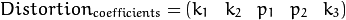
\includegraphics[scale=0.7]{Bilder/distortion.png}
	\label{fig:distortion}
\end{figure}

OpenCV betrachtet dabei radiale und tangentiale Faktoren. Die Formel für radiale Verzeichnung ist die Folgende:

\begin{figure}[ht]
	\centering
	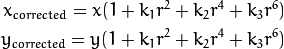
\includegraphics[scale=0.7]{Bilder/radialFactors.png}
	\label{fig:radial}
\end{figure}

Hierbei wird aus einem alten Bildpunkt $(x,y)$ des Eingabebildes die korrigierte Position $x_{corrected} y_{corrected}$ bestimmt. \newline
Die Berechnung der tangentialen Verzerrung erfolgt durch die Formel:

\begin{figure}[ht]
	\centering
	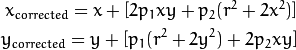
\includegraphics[scale=0.7]{Bilder/tangentialFactors.png}
	\label{fig:radial}
\end{figure}

Abschließend werden die Einheiten angepasst:

\begin{figure}[ht]
	\centering
	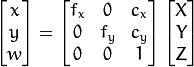
\includegraphics[scale=0.7]{Bilder/matrixEquation.png}
	\label{fig:radial}
\end{figure}

Dabei entspricht $f_x$ und $f_y$ der Brennweite der Linse und $c_x$, sowie $c_y$ beschreiben die optische Bildmitte in Pixelkoordinaten. \newline
% cite http://docs.opencv.org/2.4/doc/tutorials/calib3d/camera_calibration/camera_calibration.html
Dieser Ansatz ist der einfachste und funktioniert grundsätzlich mit jeder Kamera.

\subsubsection*{Umsetzung der Kalibrierung}
Um die intrinsischen Parameter der Kamera zu bestimmen, wird ein bekanntes Bild oder Muster aufgenommen. Dazu wird ein Vergleich zwischen den theoretischen und tatsächlichen Abmessungen angestellt. Hierzu wird meist ein einfaches Schachbrettmuster genutzt, welches im möglichst vielen verschiedenen Perspektiven aufgenommen wird. Bei der realen Drohne wird dazu das Muster ausgedruckt, bei der Simulation muss hingegen ein muss ein solches Objekt in die Welt eingefügt werden. Da die Kamera in der Simulation ohnehin keine intrinsischen Fehler aufweisen sollte, kann auf eine Kalibrierung verzichtet werden. \newline

\begin{figure}[ht]
	\centering
	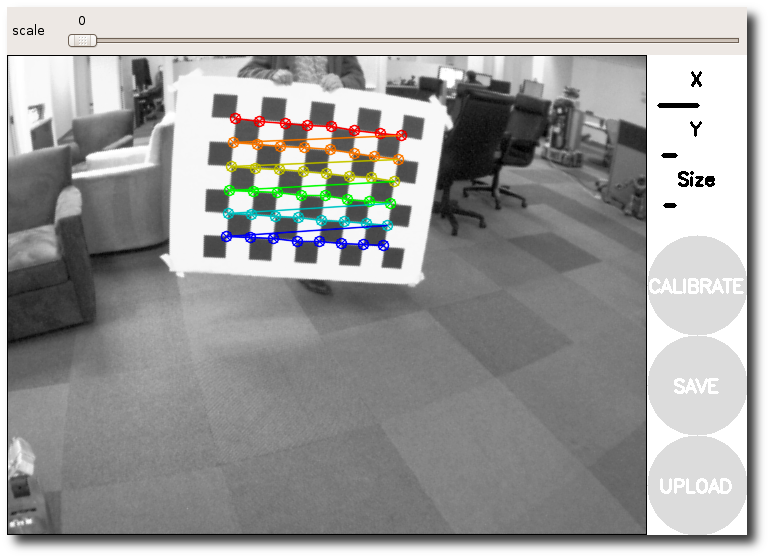
\includegraphics[scale=0.4]{Bilder/calibrationChecker.png}
	\label{fig:calibrationChecker}
\end{figure}

Die Kalibrierung wurde mit dem frei verfügbaren ROS Node \textit{camera\_calibration} umgesetzt. Das Ergebnis ist abhängig von der Anzahl der Perspektiven und der Qualität der Aufnahmen. Aufgegeben wird dann die List der Parameter, die für das Lochkamera Modell notwendig sind.

\subsection{Regularized Monocular Depth Estimation - REMODE}
%Christoph
Im vorherigen Abschnitt wurde beschrieben, wie anhand von aufeinanderfolgenden Bildern die Position der Kamera im Raum bestimmt werden kann. Dieses Problem wird seit mehr als 20 Jahren untersucht und wird als Structure From Motion \emph{SFM} in der Bildverarbeitung und Simultaneous Localization and Mapping \emph{SLAM} in der Robotik bezeichnet. \newline
%Smith, R.C.; Cheeseman, P. (1986). "On the Representation and Estimation of Spatial Uncertainty" (PDF). The International Journal of Robotics Research. 5 (4): 56–68. 
Um den Nutzer aktiv bei der Steuerung der Drohne zu unterstützen werden jedoch Tiefeninformationen benötigt. Dazu müssen Tiefenbilder und Tiefenkarten (footnote) aus den Bildern der monokularen Kamera bestimmt werden. \newline
Für diesen Schritt gibt es unterschiedliche Ansätze. Der State of the Art ist die Berechnung mit Hilfe des Bayes-Schätzers. Dabei handelt es sich um eine Schätzfunktion in der mathematischen Statistik, welche eventuell vorhandenes Vorwissen bei der Schätzung eines Parameters berücksichtigt. Dabei wird in der bayesschen Statistik das initiale Vorwissen mit Hilfe der A-priori-Verteilung modelliert, die bedingte Wahrscheinlichkeit des Parameters unter Betrachtung dieses Vorwissens mit der A-posteriori-Verteilung. \newline
%http://www.mathematik.uni-ulm.de/stochastik/lehre/ss04/statistik1/skript/node26.html
Im Umfang dieser Arbeit wird die Forschung und Implementierung des Projekts Regularized Monocular Depth Estimation \emph{REMODE} genutzt. In dieser Ausarbeitung von Matia Pizzoli, Christian Forster und Davide Scaramuzza wird die bayessche Schätzung mit neusten Entwicklungen in der Konvexoptimierung verbunden. Hierbei stützen sie ihre Forschungen auf die Ergebnisse von G. Vogiatzis und C. Hernandez und ihrer Abhandlung mit dem Titel ''Video-based, real-time multi-view stereo`` von 2011. \newline
REMODE ermöglicht eine Berechnung der Tiefeninformationen in Echtzeit und auf Pixelbasis. Weiterhin ist die aktuelle Genauigkeit und Fehlerrate im Vergleich zur Realität zu jeder Zeit sichtbar. \newline
Im Folgenden wird der grundsätzliche Ansatz der Implementierung skizziert. Die genauen Details übersteigen dabei auf Grund der hohen Komplexität den Umfang dieser Arbeit.

\begin{figure}[ht]
	\centering
	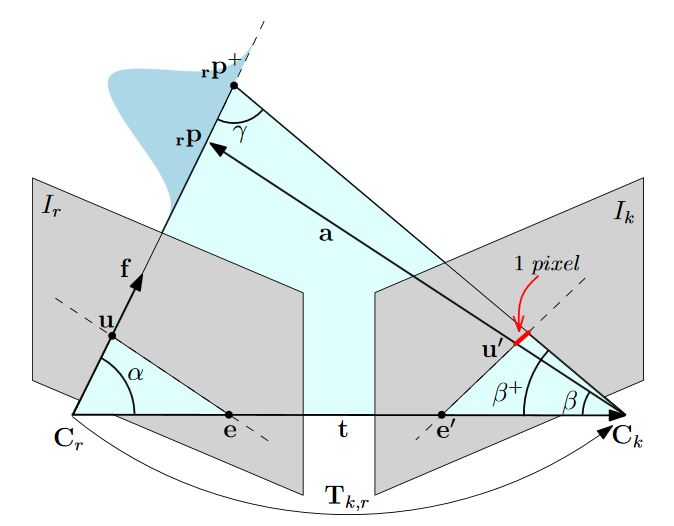
\includegraphics[scale=0.7]{Bilder/REMODE_overview.jpg}
	\label{fig:radial}
\end{figure}

In der Übersicht sieht man die beiden Kamerapositionen $I_r$ und $I_k$ mit den zugehörigen Kamerazentren $C_r$ und $C_k$. Die Positionen im Raum dieser Kameras wurden im vorherigen Schritt mit Hilfe von SVO ermittelt. $T_k,r$ zeigt dabei die starre Transformation der Kamerabilder. \newline
Der Punkt $r_P$ ist die aktuelle Schätzung der Position eines Punktes auf den epipolaren Flächen.
Die Varianz der Abweichung von einem Pixel auf der epipolaren Linie durch estrich und ustrich wird berechnet mit der Gleichung tkquadr.
Mit Hilfe der oben angesprochenen mathematischen und statistischen Auswertungen kann nun die Tiefe eines Punktes $r_P$ approximiert werden. \newline
Das Zusammenspiel von SVO und REMODE ist für handelsüblichen Laptops mit CPU und GPU ausgelegt. Dabei läuft SVO komplett auf dem Prozessor und REMODE verwendet das Framework NVIDIA CUDA, (footnote) was auf den Grafikchip des Rechners zugreift. \newline
Die Implementation setzt auf eine durchschnittliche Bewegung der Kamera von 0.0038 Meter pro Sekunde und einer mittleren Tiefe von einem Meter bei einer Berechnungszeit von 3.3 ms pro Bild.

\subsection{Performanceprobleme}
\label{performanceprobleme}
%hier mal vollkommen auslassen über alle performanceissues


\newpage
\section{Implementierung}
\subsection{Grundlegende Herausforderungen}
Es bestand eine nicht modularisierte, schlecht dokumentierte CSharp Dokumentation für eine Windowsumgebung. Diese galt es teilweise für ROS zu übernehmen. Für Windows existiert ein Kinect Software Development Kit, welches die Programmierung erleichtert.
\subsection{Kinect}

%Max
\subsection{ROS Nodes}
%Beide
\subsection{Architektur}
%Beide



%Bild der Drohne http://lightspots.ch/images/ARdronebw.png
%Bild vom Typ https://img.clipartfox.com/d02b01c31b79dd51b6c2c6a2a5db5985_stop-help-vector-art-outstretched-arm-clipart_416-416.jpeg
%Bild von kinect https://d3nevzfk7ii3be.cloudfront.net/igi/DtuTZhDHRWaOirBm.large


\newpage
\section{Assistenzsystem}
Im Kapitel \ref{Bildverarbeitung} wurde der Prozess beschrieben, wie aus den monokularen Aufnahmen der Frontkamera der Drohen Tiefenbilder ermittelt werden können. Aufbauend darauf soll nun erarbeitet werden, wie man aus diesen Informationen ein grundlegendes Assistenzsystem implementieren könnte.


\subsection{Abgrenzung}
%Christoph
Die Tiefenbilder die REMODE erstellt sind in Form von sogenannten Punktwolken, bzw. Point Clouds über ein ROS Topic verschickt. Diese Punktwolken sind eine Menge von Punkten in einem Vektorraum, welche jeweils durch ihre Raumkoordinaten in einem dreidimensionalen kartesischen Koordinatensystem beschrieben sind. Somit ist jedes Element im Datensatz durch die Attribute $X$, $Y$ und $Z$ gekennzeichnet. \newline

\begin{figure}[ht]
	\centering
	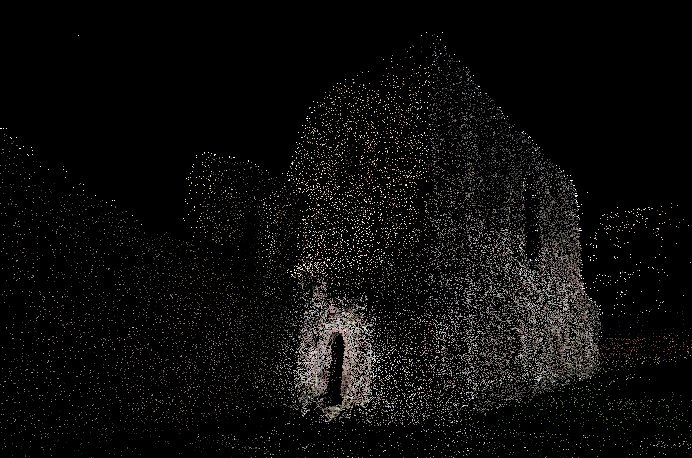
\includegraphics[scale=0.5]{Bilder/pointcloud_1.jpg}
	\label{fig:pointcloud}
\end{figure}

Die Darstellung zeigt beispielhaft die Visualisierung einer Punktwolke. Dabei entscheidet die Helligkeit der Punkte über die relative Tiefe in Bezug zur Kamera. Der Vektorraum $V \in \mathbb{R}^3$ mit den entsprechenden Datenpunkten wird über ROS Topics in einem Intervall von wenigen Sekunden übertragen.\newline
%cite https://student.myvectorworks.net/public_newsletters/2016/07/6/StudenPortal-eNL_Detail_content2.html?utm_campaign=newsletteredu&utm_source=image&utm_medium=portal&utm_content=2
%cite http://whatis.techtarget.com/definition/point-cloud
Wie zuvor beschrieben, ist ein einfacher Anwendungsfall das Fliegen durch Hindernisse wie offene Türen. Dabei stößt man in der Bildverarbeitung auf eine Reihe von Herausforderungen. Wie in \ref{performanceprobleme} beschrieben, sind SVO und REMODE nicht optimal für den Anwendungsfall dieser Arbeit. Dabei treten Probleme schon beidem ersten Schritt zum Assistenzsystem auf, die Analyse des Tiefenbildes. Dabei ist sowohl die niedrige Qualität der Tiefenbilder problematisch, als auch die hohe Zeit die zwischen der Bewegung der Drohne und der Berechnung der Tiefenpunktwolke vergehen kann. \newline
Die Folgende Darstellung zeigt ein Beispiel für ein von REMODE berechnetes Bild.

\begin{figure}[ht]
	\centering
	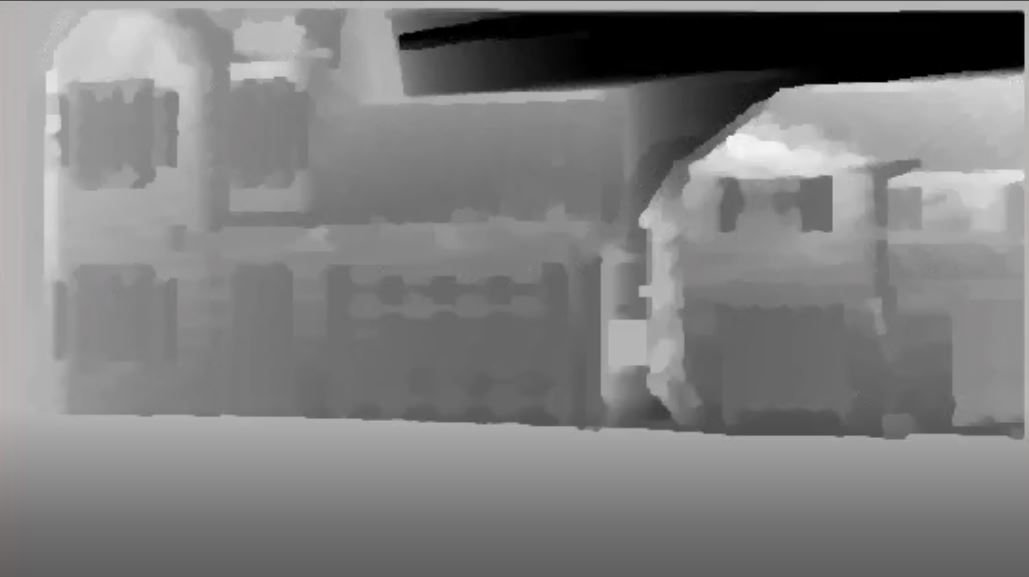
\includegraphics[scale=0.5]{Bilder/REMODE.jpg}
	\label{fig:REMODE}
\end{figure}

Dabei wird ersichtlich, das der grundlegende Kontext für einen menschlichen Betrachter verständlich ist - in diesem Fall sind dies zwei Häuser mit einer schmalen Lücke als Zwischenraum. Dabei sind genaue Texturen stark reduziert und teilweise verloren gegangen. Weiterhin sind Objektränder zum Teil von einem leichten hellen Schimmer umgeben, welcher in der Bildanalyse zu Problemen führen kann.
Um an diesem Punkt ein Objekt wie eine Tür, bzw. den Zwischenraum zu erkennen, gibt es verschiedene Ansätze, um die Punktwolke zu analysieren.
Eine Möglichkeit ist das suchen nach definierten Abmessungen, Abständen und Formen. Es ist auch möglich, die Daten mit einer Referenzpunktwolke von einem ähnlichen Objekt abzugleichen. \newline
Für beide Ansätze sind komplexe mathematische Berechnungen und Bildverarbeitungskenntnisse notwendig. Für dieses Problem gibt es das OpenSource Projekt Point Cloud Library \emph{PCL}. Dabei handelt es sich um ein Open Source Projekt zur 2D und 3D Bild-, sowie Punktwolkenverarbeitung. %cite http://pointclouds.org/
Dabei stellt die Programmbibliothek zahlreiche Algorithmen bereit, die z.B. bei der Filterung, Segmentierung und Visualisierung helfen. Dabei verfügt das Robot Operating System außerdem eine Schnittstelle zur PCL, wodurch sie sich bestens in die Projektumgebung dieser Arbeit integrieren lässt. \newline


\subsection{Implementierungsvorschlag}
%beide
%http://pointclouds.org/documentation/tutorials/correspondence_grouping.php
%vielleicht könnte das einigermaßen klappen
%falls wir nicht mehr dazu kommen wenigstens theoretische betrachtung, ob das funktionieren könnte + integration in unsere Architektur